%%%%%%%%%%%%%%%%%%%%%%%%%%%%%%%%%%%%%
% Ch2 : Les liaisons interatomiques %
%%%%%%%%%%%%%%%%%%%%%%%%%%%%%%%%%%%%%

\chapter{Liaisons interatomiques}
\section{La liaison}
	Le but des liaisons est de remplir la couche de valence et de se rapprocher au plus de la configuration des gaz rares. L'existence de composés polyatomiques stables implique que les atomes soient capable de former des agrégats dont \textbf{l'énergie est plus faible que s'ils étaient isolés}. Les types de liaison dépendent de l'agencement des électrons de valence et sont au nombre de 4 : \\

	\begin{itemize}
		\item[•] la liaison ionique
		\item[•] la liaison covalente
		\item[•] la liaison métallique
		\item[•] les liaisons secondaires hydrogène et de Vander Waals. \\
	\end{itemize}
	
	Les 3 premières sont des liaisons fortes alors que les dernières sont plus faibles. Soulignons que, le plus souvent, la liaison des atomes dans un solide présente un caractère mixte associant des contributions simultanées de plusieurs types liaisons chimiques.
	
\section{La liaison ionique, opportunisme individualiste}
	Type de liaison qui détermine la cohésion des solides constitués de l'association d'atomes possédant des affinités électronique très différentes. Prenons l'exemple du sel de cuisine $NaCl$ et regardons ce qui se passe d'un point de vue énergétique. Tout d'abord, l'énergie de première ionisation de $Na$ et l'affinité électronique (énergie libéré lorsqu'un électron est capté) de $Cl$ sont
	\begin{equation}
		E_{ion}\, Na= 5.14 \, eV \qquad et \qquad \mbox{Aff.élec } Cl = 4.02 \, eV 
	\end{equation}	 
	ce qui veut dire qu'il faut $U_i = 1.12\, eV$ pour séparer $NaCl$ en $Na^++Cl^-$. Il faut encore tenir compte de la force électrostatique $F$ entre les deux ions de charges différentes. Quand un ion se rapproche depuis l'infini, 
	\begin{equation}
		U_a = \int _\infty ^r F_{attr} \, dr= \int _\infty ^r \frac{q^2}{4\pi \epsilon _0 r^2} \, dr = -\frac{q^2}{4\pi \epsilon _0 r}
	\end{equation}
	Le signe négatif de cette énergie traduit le fait que les ions ont tendance à se rapprocher. Cependant, à très petite distance, les cortèges électroniques commencent à se superposer et une forte répulsion apparaît selon 
	\begin{equation}
		U_r = \frac{B}{r^n}
	\end{equation}
	\begin{wrapfigure}[5]{l}{6.5cm}
	\vspace{-5mm}
	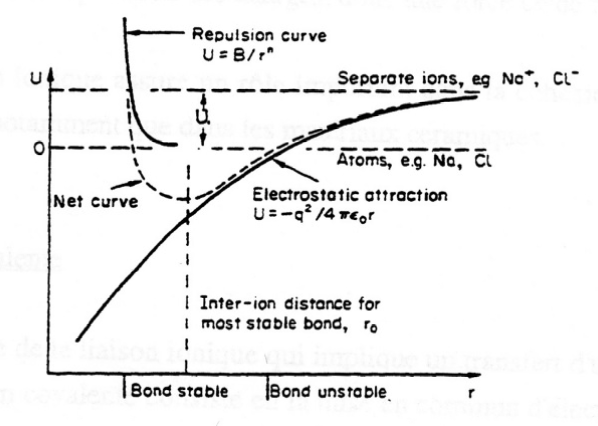
\includegraphics[scale=0.6]{ch2/1}
	\end{wrapfigure}
	La somme de toutes ces contributions donne la courbe d'énergie potentielle suivante. 
	A SUIVRE